\documentclass[10pt]{article}

\usepackage[margin=1in]{geometry}
\usepackage{amsmath,amssymb}
\usepackage{booktabs}
\usepackage{graphicx}
\usepackage{array}
\usepackage[hidelinks]{hyperref}
\usepackage{xcolor}
% Everything revised in this draft is marked in red: the move to two periods and
% the responses to the comments on the previous version. The change of
% terminology from "the disorder" to "a SUD" runs through the whole note and is
% NOT marked, since colouring every instance would colour half the document.
\newcommand{\new}[1]{\textcolor{red}{#1}}
\usepackage[official]{eurosym}
\usepackage{longtable}

\setlength{\parskip}{0.18em}
\newcolumntype{L}[1]{>{\raggedright\arraybackslash}p{#1}}

\renewcommand{\topfraction}{0.92}
\renewcommand{\bottomfraction}{0.85}
\renewcommand{\textfraction}{0.06}
\renewcommand{\floatpagefraction}{0.80}
\setlength{\textfloatsep}{12pt plus 2pt minus 3pt}
\setlength{\intextsep}{10pt plus 2pt minus 3pt}

\newcommand{\notes}[2]{\par\vspace{0.4em}%
  \begin{minipage}{#1}\footnotesize #2\end{minipage}}

\begin{document}

\begin{center}
{\Large\bfseries Housing First or Treatment First?}\\[0.35em]
{\large A stylized model, and the quantitative model behind it}\\[0.35em]
\today
\end{center}
\vspace{0.8em}


%======================================================================
\section{A stylized model}\label{sec:stylized}

%======================================================================
\subsection{Three questions}\label{sec:what}

In the data, drug use is concentrated among low income households, most of the
homeless do not carry a \new{substance use disorder (SUD)}, and housing vouchers
reach only about a quarter of the households eligible for them. The quantitative
model is built to match facts of that kind. It has six state variables and
roughly forty parameters, which is what the welfare and fiscal questions require,
but it also makes it hard to see which pieces of the environment \new{do the
heavy lifting}. This note strips the environment \new{down to help understand the
main drivers in the model, but where} my three main questions are still well
posed.

\new{Households are perfectly forward looking, here and in the quantitative model.
They face the true hazard of acquiring a SUD, they know what carrying one would
cost them, and they make no mistakes. Nothing below rests on misperception, on
myopia, or on a taste that changes once the household has used.}

\begin{enumerate}\setlength{\itemsep}{0.3em}\setlength{\parskip}{0em}

\item \textbf{Who uses drugs?} In the data, use is concentrated at the bottom of
the income distribution. \new{Drugs here are a \emph{luxury} good bought at a
price: the Stone-Geary form in equation~\eqref{eq:u} below means the share of
income spent on them rises with income, so left to itself the environment
concentrates use at the \emph{top}.} Which feature of the environment reverses
the concentration from the top to the bottom?

\item \textbf{How does housing assistance shape the drug use decision?} A
voucher pulls drug use in two opposite directions. It raises the value of
staying clean, because a housed future is worth more than a homeless one and
using puts that future at risk: call this the value of life force, and it lowers
use. In contrast, it cushions the consequence of acquiring a SUD, because
a household that acquires one is housed anyway: call this the moral hazard
force, and it raises use. Both are first order, so theory does not sign the
effect of housing assistance on drug use, and the question is quantitative.

\item \textbf{When is Treatment First better than Housing First?} In a model
without externalities, never. Housing First always raises welfare when agents
are forward looking, as they are here. A SUD creates a genuine tension,
since the same voucher that insures a household also makes the risk it insures
more attractive, but \new{that tension does not raise welfare, because Treatment
First only removes an option that a household can take under Housing First as
well}. However, if \new{a SUD} and homelessness \new{generate externalities, such
as affecting the earning potential of the children of parents with a SUD}, then
Treatment First may be preferred\new{: children of a parent with a SUD are
themselves two to four times as likely to develop one (McGovern et al., 2023),
and moving a child to a lower poverty neighbourhood before age thirteen raises
adult earnings by $31$ per cent (Chetty, Hendren and Katz, 2016)}. The
model's work here is to show why the first claim holds and then to qualitatively
price the externality that overturns it.

\end{enumerate}

The model is qualitative throughout: the calibration is rough by design, there
is no validation exercise, and every component that obscures the mechanisms has
been removed and the model refitted without it. What remains \new{are the main
drivers of the results}. The welfare evaluations below are for illustration only; the full
quantitative model is what settles the main question, which is whether Treatment
First raises welfare relative to Housing First in a model that fits the data.

%======================================================================
\subsection{The environment}\label{sec:env}

\subsubsection{Households and preferences}

\new{There are two periods and a continuum of households. A period stands for
thirty years of adult life, so the two of them span ages twenty five to eighty
five.}
Parameters with a natural annual counterpart are compounded to that length: the
discount factor is $\beta$ per period, the gross interest rate is $R=1/\beta$ so
that $\beta R = 1$, and $\phi_0$ is survival over thirty years. \new{Their values
are in Table~\ref{tab:ext} and are not repeated here.} Notation follows the
quantitative model throughout.

A household is characterised by its productivity $y$, fixed over its
life and lognormally distributed across households, $\log y \sim
\mathcal{N}(-\tfrac12\sigma^2, \sigma^2)$, so mean income is one. Households
differ in $y$, in age $j\in\{1,2\}$, in employment status $e\in\{0,1\}$, in
voucher receipt $\eta\in\{0,1\}$ and in SUD status $d\in\{0,1\}$, all
discussed below, and in nothing else.

Flow utility depends on non durable consumption $c$, housing services $h$ and
drug consumption $v$,
\begin{equation}\label{eq:u}
u(c,h,v) \;=\; (1-\gamma-\theta)\log c \;+\; \gamma \log h
\;+\; \theta\big[\log(b+v)-\log b\big] \;+\; \aleph .
\end{equation}
The three weights sum to one, so $\gamma$ is the housing budget share.
Drugs enter only in the first period, since that is the only period in which $v$
is chosen, and housing is chosen each period from a three point grid
$\{h_0,h_S,h_L\}$. The pair $(\theta,b)$ governs the drug term: the marginal
utility of the $v$th unit is $\theta/(b+v)$, so $\theta$ mostly sets how much a
user uses and $b$ whether anyone uses at all. The Stone-Geary form keeps the
first unit's marginal utility finite, \new{which is what generates non users at
all}, because under plain $\theta\log v$ every
household uses whatever the consequences. Finally $\aleph$ is the flow value of
being alive, the utility of surviving into a period over and above what is
consumed in it, which gives mortality a cost that does not vanish when
consumption is low. Households save in one risk free asset and cannot borrow.

\subsubsection{Timing}

{\color{red}
\paragraph{Period 1.} Every household is clean. Employment $e\in\{0,1\}$ is
drawn with the unemployment probability $u_0$, and a household that is income
eligible draws a voucher with probability $\pi_V$; these are the same two
lotteries it faces again in period 2. It then chooses consumption, housing, drug
use $v\ge0$, which for simplicity is the only period in which it chooses whether
to use, and saving, paying market rent $p_r$, which is normalised to one, on
whatever unit it picks. It starts with no assets. Using drugs generates the risk
of a SUD, increasing in $v$,
\begin{equation}\label{eq:hazard}
\pi(v) \;=\; 1 - e^{-\lambda v} .
\end{equation}
Because $\pi$ is increasing in $v$, the household internalises that using more
is riskier, so the intensive and extensive margins are not separate decisions.

\paragraph{The transition.} The SUD $d'\in\{0,1\}$ is realised with
probability $\pi(v)$ for households that used and with probability zero for the
rest, and the household survives into period 2 with probability
\begin{equation}\label{eq:surv}
\phi(d') \;=\; \phi_0\,(1-\kappa d'),
\end{equation}
so $\kappa$ is the proportional reduction in survival caused by the SUD.
The mortality penalty applies here, and here only.

\paragraph{Period 2.} Terminal, after which the household dies with certainty. A
household without the SUD is unemployed with probability $u_0$ and one with
the SUD with the higher probability $u_1$; if unemployed it receives income
support. The voucher is drawn again, subject to the policy rule. The household
chooses consumption and housing, there is no drug use decision, and assets are
run down with nothing bequeathed.

\paragraph{Mortality, and where the SUD is realised.} Mortality is a tax on
a continuation value, so the SUD can only cost anything if a future remains
when it is carried. That does not require a third period. It requires the
SUD to be drawn at a \emph{transition} rather than inside the terminal
period, and here it is drawn on the way into period 2, with survival over that
transition depending on it, so acquiring it puts the whole of period 2 at risk.
Realise it inside the last period instead and death costs nothing because
nothing follows it, and the mechanism the model rests on falls silent; an
earlier version of this note bought its way out of that with a third period,
which is the more expensive fix. It is also the less faithful one, since the
quantitative model draws every shock after the choices that condition it.

There is accordingly no recovery parameter here. Recovery needs a period to
recover into and period 2 is terminal, so $\rho$ has nothing to name. It belongs
to the quantitative model, where treatment is a choice and $\rho$ is the
parameter its entire effect runs through, and its absence here costs the policy
comparison nothing: what separates the two policies is whether the voucher is
withdrawn, not whether the household can get clean again.
}

\subsubsection{Employment, income support and housing}\label{sec:support}

The gap $u_1-u_0$ is the entire resource cost of the SUD. Income in a
period, given permanent productivity $y$ and employment status $e$, is
\begin{equation}\label{eq:inc}
y^{g}(y,e) \;=\;
\begin{cases}
y & \text{if } e = 1,\\[0.2em]
\psi\cdot\min\{y,\bar y\} & \text{if } e = 0,
\end{cases}
\end{equation}
with $\psi$ the replacement rate and $\bar y$ a cap on the earnings base. There
is no other income risk. The level of $\psi$ is what links the SUD to
homelessness: for the poorest households half of income can fall short of the
rent on the smallest unit, so an unemployed household there cannot house itself
out of current income.

Each period the household chooses
\begin{equation}\label{eq:opts}
h \in \{h_0,\ h_S,\ h_L\}, \qquad h_0 < h_S < h_L ,
\end{equation}
homelessness, a small unit and a standard unit. Homelessness is free and
delivers almost nothing. Two rented sizes is the fewest that lets a household
economise on housing rather than lose it: with one, homelessness comes out at
@@homeless1@@ per cent against a target of $0.40$, at any $h_0$.

A voucher covers part of the rent, is means tested and is rationed. It is drawn
independently each period, which is a simplification relative to the
quantitative model, where a voucher persists as long as eligibility holds.
Writing $\eta\in\{0,1\}$ for whether one is held,
\begin{equation}\label{eq:vouch}
\Pr(\eta'=1 \mid y', d', v) \;=\; \pi_V \cdot \mathbf{1}\{y' \le y_V\}
\cdot \mathbf{1}\{\text{policy covers } (d',v)\},
\end{equation}
and a household holding one pays the fraction $\kappa_r$ of market rent, so the
rent paid on option $j$ is
\begin{equation}\label{eq:rent}
r_j(\eta) \;=\; p_r\,h_j\big[\kappa_r \eta + (1-\eta)\big]\cdot
\mathbf{1}\{j \ne 0\},
\end{equation}
which is zero when the household is homeless. Vouchers operate in both periods,
and $\pi_V$, the share of eligible households actually covered, is the policy
dial of Section~\ref{sec:mh}.

The two policies differ in exactly one respect, the last indicator in
equation~\eqref{eq:vouch}. \textbf{Housing First} covers every eligible
household regardless of $(d',v)$. \textbf{Treatment First} covers only
households that satisfy the sobriety condition, $v=0$ and $d'=0$, which is the
rule in the quantitative model as well. Since cover in the states that follow
drug use is the only difference, the gap between them is the moral hazard and
the whole of it.

\new{The condition binds in period 1 as well, and the timing there is worth stating.
Every household arrives clean, so the period 1 voucher is drawn before $v$ is
chosen and conditionality cannot screen anyone out on entry. What it does
instead is withdraw the voucher from a household that goes on to use, within the
same period. So under Treatment First a household that uses pays market rent
immediately and again in period 2, and under Housing First it keeps what it
drew: the condition is on the choice, never on the arrival.}

\subsubsection{The household's problem}\label{sec:problem}

{\color{red}
Let $a$ be assets carried in. Period 2 is terminal, so the household consumes
everything and chooses housing,
\begin{equation}\label{eq:v2}
W_2(a,y,e,\eta,d) = \max_{j}
\Big\{ (1-\gamma-\theta)\log c + \gamma \log h_j + \aleph \Big\},
\qquad c = Ra + y^{g}(y,e) - r_j(\eta),
\end{equation}
and write $W_2(a,y,d) = \mathbb{E}\big[W_2(a,y,e,\eta,d)\mid y,d\big]$ for its
expectation over the period 2 employment and voucher draws. In period 1 the
household draws $(e,\eta)$ and then chooses housing, drug use and saving,
\begin{equation}\label{eq:v1}
V_1(y,e,\eta) = \max_{j,\,v \ge 0,\,a' \ge 0}
\Big\{ (1-\gamma-\theta)\log c + \gamma \log h_j
+ \theta[\log(b+v)-\log b] + \aleph
+ \beta\, \mathbb{E}_{d'}\Big[\phi(d')\,W_2(a',y,d')\Big] \Big\},
\end{equation}
with $c = y^{g}(y,e) - r_j(\eta) - p_v v - a'$ and $d'=1$ with the use dependent
probability of~\eqref{eq:hazard}, and $V_1(y)=\mathbb{E}[V_1(y,e,\eta)\mid y]$.

Survival sits \emph{inside} the expectation over $d'$ rather than outside it,
and that is not a matter of notation. Survival depends on the realised SUD,
so the continuation is $\mathbb{E}_{d'}[\phi(d')W_2]$ and not $\phi\,
\mathbb{E}_{d'}W_2$. Written the second way, any household whose continuation
value is negative is made better off by a lower survival probability, so it
would seek the SUD out for the mortality it brings, and the mechanism the
model rests on runs backwards. It is the same failure that makes the level of
$\aleph$ a condition to be checked rather than a free normalisation.

A household uses if the value at its best positive $v$ exceeds the value at
$v=0$. Households differ only in $y$ and in the draw $(e,\eta)$, which is the
same lottery for everyone, so within a draw the decision defines a set of income
intervals on which use occurs, and participation at a given income is the
probability of drawing a state in which the household uses.
}

%======================================================================
\subsection{Calibration}\label{sec:cal}

Table~\ref{tab:ext} lists the parameters set outside the model. Preferences and
demographics are conventional: the annual discount factor is $0.99$ and the
gross interest rate is $1/\beta$, the dispersion of log permanent income is
$\sigma = 0.75$ from Heathcote, Perri and Violante (2010), and \new{survival over
a period is $\phi_0 = @@phi0@@$, the CDC life table figure from twenty five to
fifty five}. For the SUD, the
proportional fall in survival is $\kappa = 0.45$ from Hjorth\o j et al.\ (2023),
and the two unemployment probabilities are measured directly, $u_0 = @@u0@@$
from the BLS and $u_1 = @@u1@@$ from NSDUH 2024 for respondents aged 26 and
over. Income support replaces half of previous earnings on a base capped at mean
income, in line with statutory state rules. The standard rental unit costs
$21.2$ per cent of mean income, its rent to income ratio in the ACS, and the
small unit is half of it. The voucher parameters are institutional: covered
tenants pay $30$ per cent of market rent, eligibility is capped at mean income,
and $\pi_V = 0.27$ is the HUD share of eligible households actually assisted.

Four parameters are set inside the model, in Table~\ref{tab:int}, each bracketed
on the moment it moves most rather than fitted jointly: with no preference
heterogeneity the aggregate is a cliff in $b$, so a gradient method steps out of
the region where participation is interior and walks to a corner. The flow value
of being alive $\aleph$ is matched to a value of a statistical life of @@vsl_t@@
times average annual income, about \$9 million against a mean household income of
\$113,000, which is the range surveyed by Viscusi and Aldy (2003) once their
estimates are put in current dollars. The pull of the first unit $b$ is matched
to a drug participation rate of $5.13$ per cent, housing services on the street
$h_0$ to a homelessness rate of $0.399$ per cent from the HUD point in time
counts, and the SUD hazard $\lambda$ to the $33.2$ per cent of users who
acquire a SUD.

The weight on drugs $\theta$ is set rather than calibrated, and the reason is
worth stating because the obvious alternative was tried. The natural target is
the $11$ per cent of income that users who are not addicted spend on drugs,
which the quantitative model matches, and this model cannot reach it while
keeping users poor. Two moments already pin the pair $(\lambda,v)$: the SUD
rate among users, $1-e^{-\lambda v}=0.332$, fixes $\lambda v$ at $0.403$, and an
$11$ per cent spending share on an average user income near $0.2$ would fix $v$
near $0.022$ and so $\lambda$ near $18$. Scanning $(\lambda,\theta)$ over that
region shows the model is bimodal with no interior solution: below a threshold in
$\theta$ users are the very poor and spend a hair above nothing, above it users
are the rich and the income gradient the model exists to explain is gone. The
economics is not subtle. What puts use at the bottom is that the SUD
destroys a continuation value, and for a poor household that cost is enormous
relative to the utility of the drug, so it uses as little as it can while still
using; low intensity use among the poor is the same fact as the income gradient
here, not an independent one. Setting $\theta = @@th@@$ and $\gamma =
0.25(1-\theta) = @@gam@@$, the model produces a spending share of @@dshare_m@@
per cent. It misses that moment by a wide margin, and the quantitative model,
with its separate light and heavy experimentation margins and its drug demand
from households that already carry the SUD, is where it should be matched.

\begin{table}[!tb]
\centering
\caption{Externally set parameters}\label{tab:ext}
% Generated by code/stylized/gradient.py.
\footnotesize
\begin{tabular}{@{}lllr@{}}
\toprule
Parameter & Description & Source or rationale & Value \\
\midrule
$\beta$ & Discount factor over a thirty-year period & $0.995$ annually, compounded & $0.86$ \\
$\sigma$ & Risk aversion & Standard; Attanasio and Weber (2010) & $2$ \\
$\bar\phi$ & Survival over a period, no SUD & US life table 2010, Arias (2014), ages 26--55 & $0.93$ \\
$\pi_d$ & Chance that use starts a SUD & NSDUH 2024: SUD rate over participation & $0.41$ \\
$\sigma_y$ & Dispersion of log income & SCF 2022: bottom half holds 17.2\% of earnings & $0.95$ \\
$y_{\min}$ & Income floor, over mean income & Every household values being alive & $0.24$ \\
$p_v$ & Price of a unit of drugs & Normalisation & $1.00$ \\
\bottomrule
\end{tabular}

\end{table}

\begin{table}[!tb]
\centering
\caption{Internally calibrated parameters}\label{tab:int}
% Generated by code/stylized/gradient.py.
\footnotesize
\begin{tabular}{@{}llrrr@{}}
\toprule
Parameter & Target moment & Data & Model & Value \\
\midrule
$\aleph$ & VSL over income & 80 & 80.0 & 6.60 \\
$b$ & Drug participation, NSDUH 2024 & 8.9\% & 8.9\% & 0.057 \\
$\theta$ & Drug spending over users' income & 16.0\% & 16.0\% & 0.22 \\
$\kappa_{\phi d}$ & Users' income over the average, NSDUH 2024 & 0.74 & 0.74 & 2.46 \\
\bottomrule
\end{tabular}

\end{table}

%======================================================================
\subsection{Who uses drugs}\label{sec:who}

This section asks which feature of the model puts drug use at the bottom of the
income distribution, and it starts from the force that any answer has to
overcome. Drugs are a normal good bought at a price, so a household with twice
the income gives up less utility per dollar spent on them. With no consequences
at all for acquiring a SUD that is the only force operating, and drug use
concentrates at the top: the average user then earns @@r_off@@ times the
population average.

Two features of the environment could reverse that. The \emph{mortality channel}
is that the SUD kills you, through $\kappa$ in equation~\eqref{eq:surv}.
The \emph{unemployment channel} is that it costs you a job with probability
$u_1-u_0$, and if income support cannot cover the rent you downsize, live on
less, or lose your home. Figure~\ref{fig:who} scales each from nothing to its
calibrated value, recalibrating $b$ at every point so participation stays at
$5.13$ per cent. The amount of drug use is therefore identical all along both
curves and the only thing moving is which households use.

\begin{figure}[!tb]
\centering
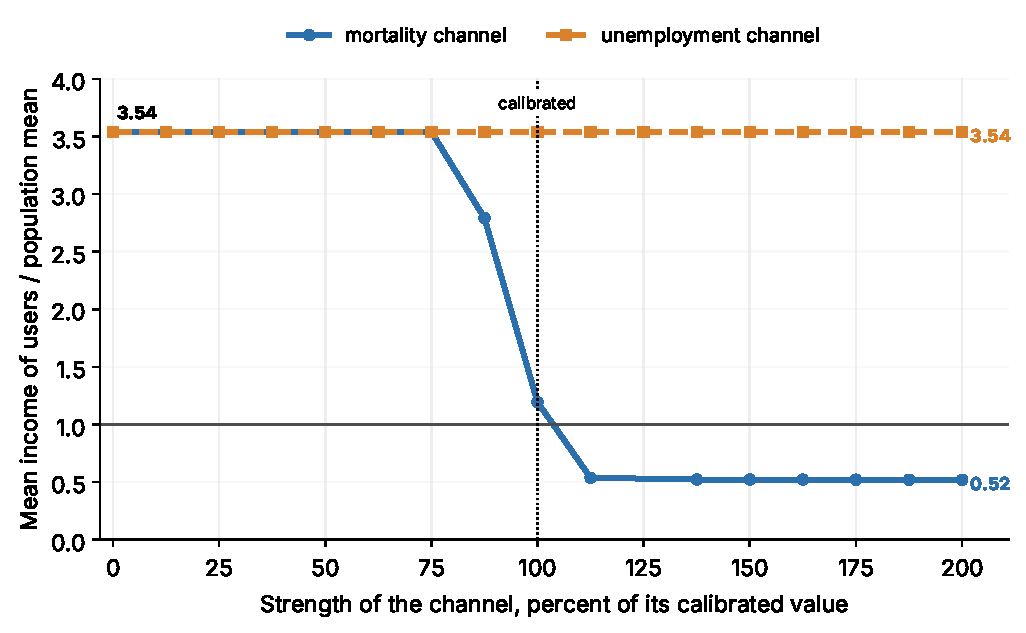
\includegraphics[width=0.62\textwidth]{figures/stylized_who_uses.pdf}
\caption{What it takes to reverse the income gradient in drug use}
\label{fig:who}
\notes{0.62\textwidth}{Note: the vertical axis is average income of users over
the population average, on a log scale, and $b$ is recalibrated at every point
so that participation is $5.13$ per cent throughout.}
\end{figure}

The result is sharper than the statement that mortality matters more. That
channel reverses the gradient at half of its calibrated strength, taking the
income ratio from @@r_off@@ to @@r_mort@@, while the unemployment channel does
not reverse it at all, leaving users at @@r_unemp@@ times average income even
fully switched on. A resource penalty cannot produce the concentration of drug
use at the bottom.

A mortality penalty is different in kind. A resource penalty scales with the
very thing it is meant to offset, since taking a fixed share of a large income
still leaves a large income, so it cannot outrun the fact that drugs are cheaper
in utility terms for the rich. What mortality destroys is not resources but a
continuation value, and the continuation value rises with permanent income. The
household with more to lose loses more, and loses proportionally more than it
gains from drugs being relatively cheap. That is the work of $\aleph$ in
equation~\eqref{eq:u}: it is the part of the continuation value that does not
shrink as consumption falls.

%======================================================================
\subsection{How does housing assistance shape the drug use decision?}\label{sec:mh}

The two forces of question 2 can be separated exactly, because they differ in
what happens to a household that uses. Under Treatment First the voucher is
withdrawn from any household that violates the sobriety condition, so only the
value of life force operates. Under Housing First it is not, so both channels
operate. Comparing the two policies at the same generosity therefore isolates
the moral hazard force, and comparing Treatment First with no programme at all
isolates the value of life force.

\begin{figure}[!tb]
\centering
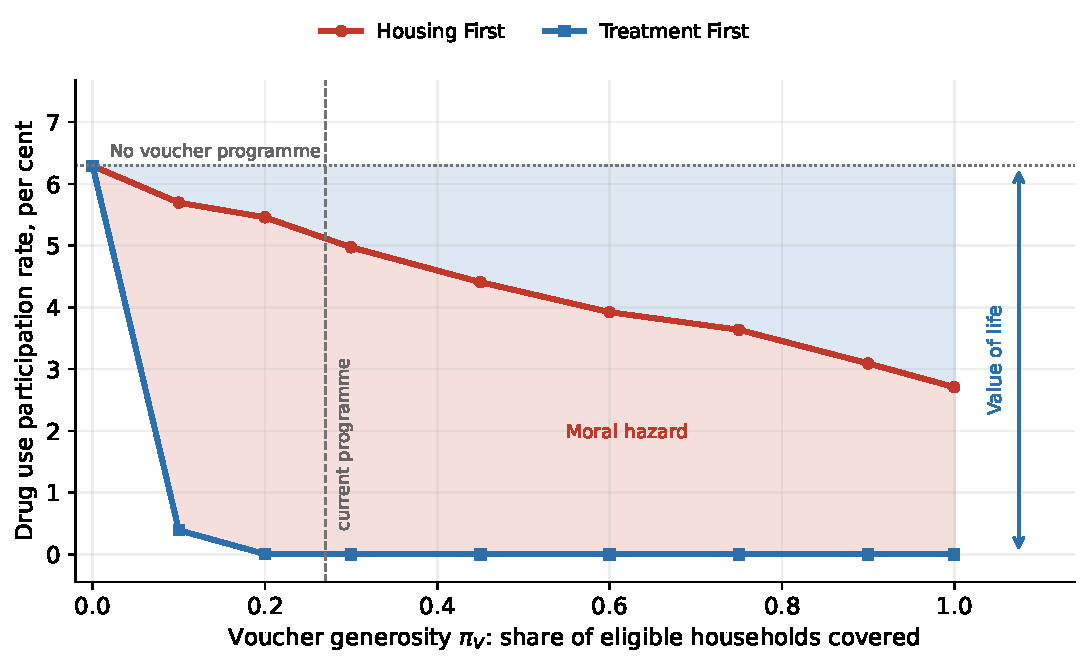
\includegraphics[width=0.66\textwidth]{figures/stylized_moral_hazard.pdf}
\caption{Drug use under the two policies as the voucher becomes more generous}
\label{fig:mh}
\notes{0.66\textwidth}{Note: the red band is the moral hazard force and the blue
band above it is what Housing First delivers net; together they are the value of
life force, marked at the right. The dashed line is the generosity of the
current programme, $\pi_V = 0.27$.}
\end{figure}

Figure~\ref{fig:mh} traces both as generosity rises. With no programme at all,
@@p0@@ per cent of households use. Universal Treatment First takes that to
@@pt@@ per cent, a value of life force of @@vol@@ percentage points; universal
Housing First leaves it at @@ph@@ per cent, so the moral hazard force is
@@mh@@ points and the net effect of Housing First is @@net@@. Both forces are
first order and they work against each other, which is the central feature of
the problem. Anyone asserting that housing the homeless must increase drug use,
or must reduce it, is making a quantitative claim that needs to be tested.

Figure~\ref{fig:margins} plots the homelessness and SUD outcomes for each
programme as its generosity changes, alongside drug use. On homelessness the two
policies end in the same place, both driving it from @@hl0@@ per cent with no
programme to zero, and along the way Treatment First is if anything slightly
below Housing First, because the households it deters from using never acquire
the SUD that puts their housing at risk. The larger difference is on the
other margin, where at universal cover Housing First leaves @@sudh@@ per cent of
the population carrying the SUD and Treatment First leaves @@sudt@@ per
cent. What the moral hazard buys is extra SUD cases among households that
are housed either way.

\begin{figure}[!tb]
\centering
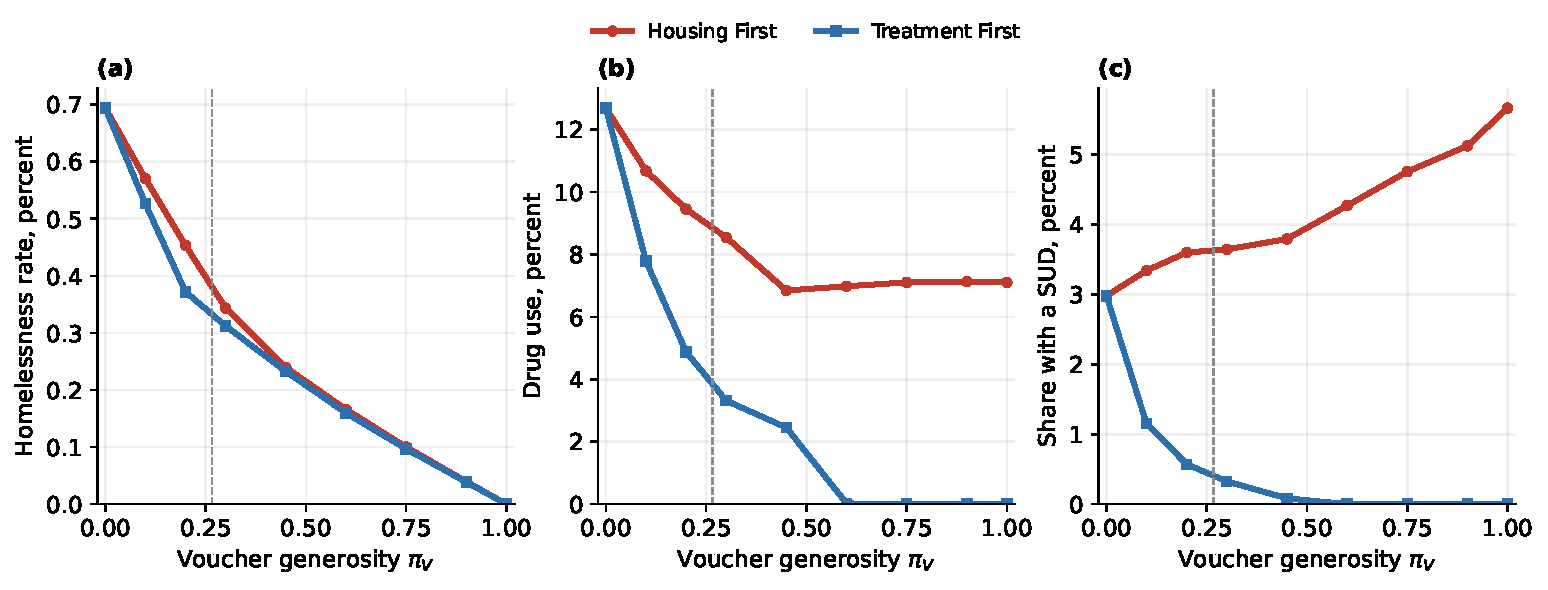
\includegraphics[width=0.88\textwidth]{figures/stylized_margins.pdf}
\caption{Homelessness, drug use and the SUD under the two policies}
\label{fig:margins}
\end{figure}

%======================================================================
\subsection{Welfare}\label{sec:welfare}

\subsubsection{Without externalities, Housing First always wins}\label{sec:nox}

Sections~\ref{sec:who} and~\ref{sec:mh} establish what each policy does to
behaviour. This section asks what each does to welfare, comparing the two at the
same generosity $\pi_V$, whose outcomes are in Panel A of
Table~\ref{tab:welfare}. The policies differ only in the last indicator in
equation~\eqref{eq:vouch}, so Housing First transfers resources in a superset of
the states in which Treatment First does. The budget set is weakly larger in
every state and strictly larger in one, so a household that optimises cannot be
worse off:
\begin{equation}\label{eq:dom}
V_1(y;\ \text{HF},\ \pi_V) \;\ge\; V_1(y;\ \text{TF},\ \pi_V)
\qquad \text{for every } y,
\end{equation}
with equality exactly for households that never use. Put the other way round, a
household under Housing First can reproduce its Treatment First outcome exactly
by not using: conditionality removes an option from a forward looking optimiser
and gives nothing back. This is a dominance argument, not a calibrated result,
and no choice of parameters overturns it.\footnote{The same comparison in the
quantitative model gives the same answer.}

It follows that the moral hazard is not a distortion. Households here face the
true SUD hazard and make no mistakes, so the extra use Housing First
induces is not a wedge to be closed but a household optimally taking a risk it
is now better able to bear. The @@mh@@ points of Section~\ref{sec:mh} are a
statement about drug use and not about welfare. Panel B of
Table~\ref{tab:welfare} puts numbers on it: @@worse@@ per cent of households are
strictly worse off under Treatment First, none is better off, and those affected
lose @@cev_aff@@ per cent of consumption.

\begin{table}[!tb]
\centering
\caption{Welfare at universal cover, with no externality}\label{tab:welfare}
\small
\begin{tabular}{@{}lcc@{}}
\toprule
& Housing First & Treatment First \\
\midrule
\multicolumn{3}{@{}l}{\emph{Panel A. Outcomes at universal cover}} \\
\quad Drug participation rate & 9.21\% & 0.00\% \\
\quad Share with a SUD & 9.209\% & 0.000\% \\
\quad Homelessness rate & 0.000\% & 0.000\% \\
\quad Voucher outlay per household & 0.0858 & 0.0851 \\
\addlinespace
\multicolumn{3}{@{}l}{\emph{Panel B. Treatment First against Housing First, no externality}} \\
\quad Households strictly worse off & & 10.1\% \\
\quad Households strictly better off & & 0.0\% \\
\quad Consumption equivalent, those affected & & 0.62\% \\
\quad Consumption equivalent, whole population & & 0.063\% \\
\bottomrule
\end{tabular}

\notes{0.9\textwidth}{Note: the consumption equivalent is the proportional change
in consumption, in every period and state, worth as much as the difference in
lifetime value. Voucher outlay is expected spending on a household from period 2
on, discounted, per unit of average income.}
\end{table}

A fixed budget does not rescue conditionality either. Treatment First is
actually slightly \emph{more} expensive at universal cover, @@costt@@ against
@@costh@@, so matching on cost rather than on generosity changes nothing. The
reason is that \new{survival into period 2 falls from @@phi0@@ to @@phi1@@ with a
SUD, so the households the moral hazard adds to the rolls die sooner and
draw voucher payments in fewer states}. So a case for conditionality has to come
from an externality.

\subsubsection{The externality on children reverses it}\label{sec:kids}

\begin{table}[!tb]
\centering
\caption{The externality on children}\label{tab:children}
\footnotesize
\begin{tabular}{@{}lcccc@{}}
\toprule
\multicolumn{5}{@{}l}{\emph{Panel A. Transmission: what each income penalty implies}} \\
$\delta_d$ &  & Child's SUD rate & Ratio & CEV \\
\midrule
0.00 &  & \textcolor{red}{6.06\%} & 1.00 & 0.0\% \\
0.20 &  & \textcolor{red}{8.94\%} & \textcolor{red}{1.47} & 41.2\% \\
0.54\ \ (calibrated) &  & \textcolor{red}{18.19\%} & \textcolor{red}{3.00} & \textcolor{red}{216.5\%} \\
0.60 &  & \textcolor{red}{20.92\%} & \textcolor{red}{3.45} & \textcolor{red}{280.8\%} \\
\addlinespace
\multicolumn{5}{@{}l}{\emph{Panel B. Does the externality reverse the ranking?}} \\
\quad Private cost of conditionality &  &  &  & \textcolor{red}{0.090\%} \\
\quad Disorder cases prevented &  &  &  & \textcolor{red}{7.624 pp} \\
\quad CEV to the child, one case &  &  &  & \textcolor{red}{202.6\%} \\
\quad Externality gain from conditionality &  &  &  & \textcolor{red}{15.446\%} \\
\quad Gain over loss &  &  &  & \textcolor{red}{170.9} \\
\bottomrule
\end{tabular}

\notes{0.82\textwidth}{Note: Panel A is at the baseline programme, $\pi_V=0.27$,
since the transmission ratio in the data comes from an economy with a rationed
programme; Panel B is at universal cover, one child per household, no
discounting across generations. Losses are consumption equivalents.}
\end{table}

The externality I model is one that runs through income rather than through
preferences. I have considered two alternatives, but both seem to be at odds
with reality. Letting the child of a user inherit a stronger taste, a lower $b$,
matches the transmission fact but has the wrong welfare sign: $b$ enters only
through $\theta\log(1+v/b)$, so a lower one raises the child's objective at every
$v>0$ and its lifetime value with it. Letting it inherit a greater
susceptibility, a higher $\lambda$, fails the other way, since a child facing a
riskier drug optimally uses \emph{less} and is worse off ex ante, which is
clearly counterintuitive.

Income works on both counts, and it works through the channels explored in
Section~\ref{sec:who}: lower permanent income is unambiguously bad to receive,
and this model already puts users at the bottom, so a child born poorer is
mechanically more likely to use, which is aligned with the data. The income
gradient does the whole job, so the model transmits a SUD across generations
\emph{without transmitting any preference for drugs}.

A child's baseline income is drawn from the same lognormal as everyone else, and
the entire link is the penalty
\begin{equation}\label{eq:kids}
y_{\text{child}} \;=\; y_{\text{base}}\,
(1-\delta_d)^{\mathbf{1}\{\text{parent acquired the SUD}\}}\,
(1-\delta_h)^{\mathbf{1}\{\text{parent was homeless}\}} ,
\end{equation}
which the parent does not internalise. That is what makes it an externality
rather than something already priced into $V_1$.

The two penalties are set to different things. Panel A of
Table~\ref{tab:children} shows that $\delta_d = 0.30$ makes the child of a
parent who acquired the SUD @@ratio@@ times as likely to acquire one, in
the middle of the epidemiological range of two to four in McGovern et al.\
(2023) and the alcohol literature. The homelessness penalty $\delta_h$ is set
directly from Chetty, Hendren and Katz (2016), who find that children who moved
to a low poverty neighbourhood before age 13 went on to earn $31$ per cent more
as adults. The two penalties also do different work: both policies drive
homelessness to zero at universal cover, so $\delta_h$ prices the programme
against no programme while $\delta_d$ decides Treatment First against Housing
First.


Panel B puts the two sides together and they are not close. The private cost of
conditionality, in the first row, is @@priv@@ per cent of consumption, small
because only @@worse@@ per cent of households are affected. Against that,
conditionality prevents @@dsud@@ percentage points of SUD cases in the
second row, and each of those cases costs one child @@percase@@ per cent of
consumption, in the third. The externality gain is @@ratiogl@@ times the private
loss, and stays above it throughout the range of $\delta_d$ in Panel A. Housing
First is better for every household taken one at a time, and worse once one
counts the children of the households it fails to deter.

Treatment First drives drug use to \emph{exactly} zero here, and that inflates
the margin. Nobody in this model faces the sobriety condition and fails to meet
it, and the households who cannot comply are the entire empirical case for
Housing First.

The point of this section is only that an externality can reverse a ranking that
is otherwise airtight, and one externality is enough to show it. Which way the
comparison actually goes is a question about magnitudes, and that is what the
quantitative model is for.

%======================================================================
\section{The quantitative model}\label{sec:full}

This section states the model the paper's numbers come from, completely. Where
the stylized model already carries something unchanged it is named rather than
motivated a second time: the Stone-Geary form of the drug term, the logic that
separates the two policies, and the transmission externality all appear below
exactly as Sections~\ref{sec:env} to~\ref{sec:kids} give them. Everything else is
written out, because it is what turns a directional answer into a quantitative
one.

\subsection{Demographics, the state and the choice set}

Households enter at age $26$, live at most to $85$, so $j=1,\dots,J=60$ annual
periods, and retire at $j_R=41$. Survival from $j$ to $j+1$ is $\phi_j(h',d,m)$
in~\eqref{eq:fsurv}: it depends on age, on the housing \emph{chosen} this period,
on the SUD and on mental illness. Newborns replace the dead. The individual
state is
\begin{equation}\label{eq:fstate}
s=(a,\,y,\,e,\,d,\,m,\,\eta)\in
\mathcal A\times\mathcal Y\times\{1,2,3\}\times\{0,1\}^3 ,
\end{equation}
assets $a\ge0$ on a \new{$50$} point grid dense near zero, permanent productivity
$y$ on $9$ points, employment $e$, the SUD $d$, serious mental illness $m$ and
the voucher $\eta$, which is \new{$10{,}800$} points per age and
\new{$648{,}000$} in total.

Two economies in that list are choices rather than oversights. \new{There are two
employment statuses, employed and unemployed. Unemployment insurance is paid for
the first year of a spell and nothing after it, so a household in its first year
of unemployment and one in its third have different income and different
continuation values and cannot be merged; $e$ therefore takes three values, the
third being an unemployment duration marker rather than a third status. There is
no probability of receiving insurance: it used to be drawn on entry into a spell,
and that parameter is gone, which removes a parameter without removing a state.}
And the housing unit a
household arrives in is not a state: everything that conditions on housing
conditions on the unit chosen, and renters face no adjustment cost, so carrying it
would replicate the whole problem four times over for nothing. It would have to be
reinstated if moving costs were added.

Each period the household chooses
\begin{equation}\label{eq:fchoice}
\big(n,\,h',\,v,\,\tau,\,a'\big)\in
[0,1]\times\{h_1,h_2,h_3,h_4\}\times\mathbb R_+\times\{0,1\}\times\mathcal A ,
\end{equation}
hours $n$, housing $h'$ where $h_1$ is homelessness, drug use $v$, treatment take
up $\tau$, available only when $d=1$, and next period assets $a'$. Every shock is
drawn \emph{after} all of that, which is what makes those variables state
variables rather than choices, and it is why the transitions in
Section~\ref{sec:fshocks} condition on the chosen $h'$, $v$ and $\tau$: the choice
comes first, the draw second.

\subsection{Preferences}

Period utility is
\begin{equation}\label{eq:futil}
u\big(c,h',v,n,\tau;d,m\big) \;=\;
\frac{\big[\,c^{\alpha}\,(h')^{\beta}\,(v+b_{dmh'})^{\gamma}\,\big]^{1-\sigma}}{1-\sigma}
\;+\;\omega_{\ell}\frac{(1-n)^{1-\sigma_{\ell}}}{1-\sigma_{\ell}}
\;+\;\aleph\;-\;\tau\bar\tau^{u}\;-\;\kappa_x\big(H+\omega_x H_D\big),
\end{equation}
with $\alpha+\beta+\gamma=1$. Equation~\eqref{eq:u} is the logarithmic case of the
bundle with hours fixed, so $\gamma$ and $b$ do what $\theta$ and $b$ do in
Section~\ref{sec:env}: $b$ is the Stone-Geary endowment that keeps the marginal
utility of the first unit finite and therefore decides whether anyone uses at all.

Four things are new. Leisure makes hours a margin. Treatment costs utility rather
than money, which is what the evidence supports, since the three largest barriers
reported in the NSDUH are beliefs and preferences and not prices. The term
$\kappa_x(H+\omega_x H_D)$ prices the disamenity of the aggregate homelessness
rate $H$, weighted by the share $H_D$ carrying the SUD; it is zero in the
benchmark, for the reason Section~\ref{sec:fleftout} gives. And the Stone-Geary
shifter itself varies,
\begin{equation}\label{eq:fb}
b_{dmh'}=b_d\cdot\rho_m^{\mathbf{1}\{m=1\}}\cdot\rho_H^{\mathbf{1}\{h'=h_1\}},
\qquad \rho_m,\rho_H\in(0,1],
\end{equation}
so the SUD, mental illness and homelessness each raise the marginal utility
of the first unit of the drug. The Cobb-Douglas weights themselves are held fixed
across the SUD: only the shifter moves. This matters for what follows,
because $\rho_H<1$ is one of the four channels through which homelessness and the
SUD reinforce each other.

\subsection{Income, taxes and transfers}

Gross income depends on age, employment, productivity and health,
\begin{equation}\label{eq:fincome}
y^{g}(j,y,e,d,m,n)=
\begin{cases}
0.40\,y & j\ge j_{R} \quad\text{(social security)}\\[2pt]
n\,y\,\varepsilon_j\,\rho_{d}^{\mathbf{1}\{d=1\}}\rho_{m}^{\mathbf{1}\{m=1\}}
 & j<j_{R},\ e=1 \quad\text{(employed)}\\[2pt]
\new{\min\{\varrho_{UI}\,y\,\varepsilon_j,\ \bar u\,\bar Y\}}
 & j<j_{R},\ e=2 \quad\text{\new{(first year of a spell)}}\\[2pt]
\zeta_{DI}\,\bar y_{DI}\,\bar Y & j<j_{R},\ e=3,\ m=1 \quad\text{(disability)}\\[2pt]
0 & \text{otherwise,}
\end{cases}
\end{equation}
with $\varepsilon_j$ the deterministic age profile of efficiency, $\rho_d$ and
$\rho_m$ productivity penalties applied \emph{conditional on working},
$\varrho_{UI}$ the replacement rate paid on the household's own productivity, up
to \new{a cap $\bar u$ on the benefit as a share of average income, as in
equation~\eqref{eq:inc},}
$\zeta_{DI}$ the share of the non employed with mental illness who receive
disability, and $\bar Y$ average income. Retirement income replaces $40$ per cent
of the productivity state with no health penalty, since social security is not
means tested on health.

The conditioning of the penalties on \emph{working} is what lets an employed
household be poor enough to choose homelessness. An unemployment effect alone
cannot do that, and the data require it: the homeless are roughly half in work,
not none. Section~\ref{sec:support}'s environment, where only unemployment
lowers income, is exactly the version that cannot.

Labour income is taxed with the Heathcote, Storesletten and Violante function and
capital income at a flat rate,
\begin{equation}\label{eq:ftax}
y^{n}=\tau_{\ell}\,(y^{g})^{\xi}\;+\;(1-\tau_k)\,r\,a ,
\end{equation}
where $\xi$ governs progressivity and $\tau_{\ell}$ the level, and $\tau_{\ell}$
is what clears the government budget. Two transfers follow, both means tested on
gross income as the programmes themselves are. A food stamp floor tops means
tested income up to $\underline c\,\bar Y$, and the voucher covers rent above a
tenant contribution of $\kappa_r$ of gross earnings,
\begin{equation}\label{eq:ftrans}
F=\max\big\{0,\ \underline c\,\bar Y-(y^{g}+\max\{0,ra\})\big\},
\qquad
V\!ch=\mathbf{1}\{\eta=1\}\,\mathbf{1}\{h'\neq h_1\}\,
\max\big\{0,\ p_h h'-\kappa_r\,y^{g}\big\}.
\end{equation}
A homeless voucher holder does not lose the voucher: retention depends on income
eligibility, not on housing, so the entitlement survives and simply pays nothing
until the household rents again.

\subsection{The budget constraint and the hours choice}

\begin{equation}\label{eq:fbudget}
c+p_v v+a' \;=\; y^{n}+a\;-\;p_h h'\,\mathbf{1}\{h'\neq h_1\}\;+\;V\!ch+F,
\qquad c>0,\ v\ge0,\ a'\ge0 .
\end{equation}
Note what is absent: treatment, which costs utility, and bequests, which go to
the government. Given $a'$ and $h'$, write $R$ for the resources left over.
Cobb-Douglas preferences over $(c,v+b)$ split them in closed form,
\begin{equation}\label{eq:fcv}
c=\frac{\alpha}{\alpha+\gamma}\big(R+p_v b_{dmh'}\big),
\qquad
v=\max\Big\{0,\ \frac{\gamma}{(\alpha+\gamma)p_v}\big(R+p_v b_{dmh'}\big)-b_{dmh'}\Big\},
\end{equation}
so the inner allocation never needs a numerical search, and the corner in $v$ is
where the household abstains because the Stone-Geary endowment already exceeds
its desired intake. That is how a large $b$ deters use, and it is the same
mechanism as the threshold in Section~\ref{sec:problem}.

Hours solve
\begin{equation}\label{eq:ffoc}
u_c(c)\,\frac{\partial R}{\partial n}\;=\;\omega_{\ell}(1-n)^{-\sigma_{\ell}} .
\end{equation}
The clawbacks in~\eqref{eq:ftrans}, at a rate of one for food stamps and
$\kappa_r$ for the voucher, make $\partial R/\partial n$ jump \emph{up} at the
hours where each transfer is exhausted, because the clawback stops. The residual
is therefore not monotone in $n$ and~\eqref{eq:ffoc} can have several roots, so
it is solved by comparing the candidate roots rather than by a first order
condition alone. This is the welfare trap, and it is the channel through which
conditionality changes labour supply rather than only consumption.

\subsection{Housing, and the homelessness loop}

Housing is a four point grid. $h_1$ is literal homelessness, sleeping rough or in
an emergency shelter, which is the HUD point in time definition and excludes
doubling up; it carries a small service flow and no rent. The three rental sizes
are geometric,
\begin{equation}\label{eq:fhouse}
h_2=\underline h,\qquad h_3=\underline h\,\varsigma,\qquad h_4=\underline h\,\varsigma^{2},
\end{equation}
so two parameters describe the grid. Rent $p_h$ is normalised to one and the
\emph{grid} is the calibrated object, since rescaling the grid by $\lambda$ and
the price by $1/\lambda$ leaves every budget constraint untouched and identifying
the level would run through a weak channel.

Homelessness then enters four separate equations: survival~\eqref{eq:fsurv},
the employment transitions~\eqref{eq:femp}, the recovery
hazard~\eqref{eq:frecover} and the Stone-Geary shifter~\eqref{eq:fb}. It raises
mortality, worsens both employment margins, lowers the chance of recovering, and
raises the marginal utility of the drug. Those four together are what make
homelessness and the SUD mutually reinforcing rather than merely correlated,
and it is that loop, absent from Section~\ref{sec:env}, that a housing programme
acts on.

\subsection{Drug use, the SUD, recovery and treatment}

A household either abstains or uses, with $v$ chosen continuously
by~\eqref{eq:fcv}. A clean household that uses acquires the SUD with the
hazard of equation~\eqref{eq:hazard},
\begin{equation}\label{eq:fd}
\Pr(d'=1\mid d=0,v)=\pi_d(v)=1-e^{-\lambda v},
\end{equation}
a single hazard rising in the quantity used, with no light and heavy split and no
threshold, so as in Section~\ref{sec:env} the intensive and extensive margins are
not separate decisions. A household with the SUD recovers with probability
\begin{equation}\label{eq:frecover}
\pi_r(h',\tau,m)=\min\Big\{1,\ \bar\pi_r\,
\mu_H^{\mathbf{1}\{h'=h_1\}}\,\mu_m^{\mathbf{1}\{m=1\}}\,g^{\tau}\Big\},
\end{equation}
with $\mu_H<1$, recovery is harder on the street, $\mu_m<1$, harder with mental
illness, and $g>1$ the treatment effect.

Treatment $\tau$ is a \emph{choice}, not a mechanical hazard, taken at the utility
cost $\bar\tau^u$ in~\eqref{eq:futil}. This matters more than it looks: the policy
under evaluation is called Treatment First, and $g$ is the parameter through
which its entire effect runs, so treatment has to be something a household decides
to undertake and can decline. Section~\ref{sec:mh}, where the only margin is
whether to use, has no counterpart for it.

\subsection{Serious mental illness}

$m$ is an exogenous two state Markov chain representing \emph{serious} mental
illness, about $5.5$ per cent of adults, defined by substantial functional
impairment, rather than any mental illness, which is roughly a quarter of adults
and includes mild anxiety: a state that halves productivity cannot sensibly cover
a quarter of the population. The onset rate is derived from the target prevalence
$p_m$ and the recovery rate $\lambda_m$,
\begin{equation}\label{eq:fonset}
\text{onset}_m=\lambda_m\frac{p_m}{1-p_m},
\qquad
\Pr(m'=1\mid m=0,d)=\text{onset}_m\cdot\iota^{\mathbf{1}\{d=1\}},
\qquad
\Pr(m'=0\mid m=1)=\lambda_m,
\end{equation}
so calibrating persistence never disturbs prevalence, and $\iota>1$ makes the
SUD raise the hazard of mental illness. That last channel runs in the
direction the evidence supports: substance induced psychosis converts to
schizophrenia or bipolar disorder at a pooled rate near a quarter, and in the
Danish registers any SUD predicts conversion to schizophrenia
with a hazard ratio of $1.34$, opioid use disorder $2.74$.

Mental illness then affects six objects: productivity conditional on working
through $\rho_m$ in~\eqref{eq:fincome}, both employment margins through
$\kappa_{uem}$, mortality through $\kappa_{\phi m}$, the recovery hazard through
$\mu_m$, the Stone-Geary shifter through $\rho_m$ in~\eqref{eq:fb}, and
eligibility for disability income through $\zeta_{DI}$.

The mental health chain does \emph{not} depend on housing, and that is a result
rather than an omission. In the At Home / Chez Soi randomised trial, $1{,}198$
homeless adults with mental illness across four cities, assignment to housing
with intensive case management produced no detectable effect on symptom severity
at any wave, while producing large effects on housing stability, its primary
outcome. Making the channel housing dependent would mean adding a mechanism the
best available trial looked for and did not find.

\subsection{What the SUD and homelessness cost}

Survival is
\begin{equation}\label{eq:fsurv}
\phi_j(h',d,m)=1-\min\Big\{1,\ (1-\bar\phi_j)\,
\kappa_{\phi H}^{\mathbf{1}\{h'=h_1\}}\,\kappa_{\phi d}^{\mathbf{1}\{d=1\}}\,
\kappa_{\phi m}^{\mathbf{1}\{m=1\}}\Big\},
\end{equation}
with $\bar\phi_j$ the baseline age profile and the multipliers themselves varying
with age, rather than the single $\kappa$ of~\eqref{eq:surv}. Because $\aleph>0$ a
higher death hazard is a real cost, and it is larger for households with more life
remaining and more to consume, which is precisely the sorting
Section~\ref{sec:who} isolates.

Job finding and separation are
\begin{equation}\label{eq:femp}
\pi^{ue}=\min\Big\{1,\ \bar\pi^{ue}\,\kappa_{ueH}^{\mathbf{1}\{h'=h_1\}}
\kappa_{ued}^{\mathbf{1}\{d=1\}}\kappa_{uem}^{\mathbf{1}\{m=1\}}\Big\},
\qquad
\pi^{eu}=\min\Big\{1,\ \bar\pi^{eu}\,\kappa_{ueH}^{-\mathbf{1}\{h'=h_1\}}
\kappa_{ued}^{-\mathbf{1}\{d=1\}}\kappa_{uem}^{-\mathbf{1}\{m=1\}}\Big\},
\end{equation}
so each multiplier below one makes work simultaneously harder to find and easier
to lose. In the baseline there is no direct wage penalty conditional on working,
$\rho_d=1$: the robust findings are on the employment margin, roughly half again
as much unscheduled absence and $44$ per cent higher turnover, while the wage
penalty conditional on working is contested. A version calibrated to the income
ratio of those with the SUD is reported as an alternative.

\subsection{The voucher, and the two policies}

A household without a voucher draws one with probability $\pi_V$ if it is income
eligible, and a household with one keeps it while eligible, so unlike
Section~\ref{sec:support} the voucher is persistent rather than redrawn each
period. Eligibility is
\begin{equation}\label{eq:felig}
y^{g}+\max\{0,ra\}\;<\;\kappa_V\cdot\text{median income}.
\end{equation}
Under Housing First that is the whole rule. Under Treatment First the voucher is
additionally lost with probability $p_{\text{det}}$ by a household that used and
with probability $p_{\text{fp}}$ by one that did not,
\begin{equation}\label{eq:fpol}
\Pr(\eta'=1)=\Pr(\eta'=1)^{HF}\times
\begin{cases}
1-p_{\text{det}} & \text{if } v>0,\\
1-p_{\text{fp}} & \text{if } v=0 .
\end{cases}
\end{equation}
This is the one place where the quantitative model changes the \emph{logic} of
Section~\ref{sec:mh} rather than its setting. There, conditionality is perfectly
enforced and perfectly met, so Treatment First deters everyone and nobody is
thrown off the rolls. Here detection is imperfect and so are households: some fail
the condition because they cannot get clean, and some fail it because the test is
wrong. Those two groups are the empirical case for Housing First, neither exists
in the stylized model, and that is why its welfare numbers are illustration.

\subsection{The shocks, collected}\label{sec:fshocks}

Conditional on the state and the choices, next period's state is drawn from five
independent transitions. Collecting them in one place:

\paragraph{Productivity $y$.} Fixed over the life cycle. It carries the cross
sectional dispersion of permanent income and the intergenerational link, and it
is a type rather than a process, so $y'=y$. This is a departure from the
submitted paper, where $y$ followed a persistent autoregression, and it is made
for two reasons: it is what keeps the child's penalty~\eqref{eq:fnewborn} a shift
along a single scalar rather than a shift across the nodes of an age varying
discretisation, and unemployment is the income risk that links the SUD to
housing, which is retained in full. The stochastic version is the robustness
direction.

\paragraph{Employment $e$.} \new{A household that separates receives insurance
with certainty for one year, so with $\pi^{ue}$ and $\pi^{eu}$
from~\eqref{eq:femp},}
\begin{equation}\label{eq:fetrans}
e=1\ \longrightarrow
\begin{cases}
e'=1 & \text{w.p. } 1-\pi^{eu}\\
e'=2 & \text{w.p. } \pi^{eu}
\end{cases}
\qquad
e\in\{2,3\}\ \longrightarrow
\begin{cases}
e'=1 & \text{w.p. } \pi^{ue}\\
e'=3 & \text{w.p. } 1-\pi^{ue},
\end{cases}
\end{equation}
\new{which is where insurance lasting exactly one year comes from: state $2$ is
entered only from employment and is never entered from itself, so the second year
of a spell is state $3$ and pays nothing.}

\paragraph{The SUD $d$.} By~\eqref{eq:fd} if $d=0$ and~\eqref{eq:frecover}
if $d=1$, conditioning on the chosen $v$, $h'$ and $\tau$.

\paragraph{Mental illness $m$.} By~\eqref{eq:fonset}, conditioning on $d$.

\paragraph{The voucher $\eta$.} By~\eqref{eq:felig} and~\eqref{eq:fpol},
conditioning on next period's eligibility and, under Treatment First, on the
chosen $v$.

Write $\Gamma\big(s'\mid s,\,n,h',v,\tau\big)$ for the product of these five,
which is the object the expectation in~\eqref{eq:fbellman} is taken against.

\subsection{The household's dynamic problem}

Putting it together, for $j=1,\dots,J$ and with $V_{J+1}$ given below,
\begin{equation}\label{eq:fbellman}
\begin{aligned}
V_j(a,y,e,d,m,\eta)=\max_{\,n,\,h',\,v,\,\tau,\,a'}\ \Bigg\{\
&\frac{\big[c^{\alpha}(h')^{\beta}(v+b_{dmh'})^{\gamma}\big]^{1-\sigma}}{1-\sigma}
+\omega_{\ell}\frac{(1-n)^{1-\sigma_{\ell}}}{1-\sigma_{\ell}}
+\aleph-\tau\bar\tau^{u}-\kappa_x\big(H+\omega_x H_D\big)\\[2pt]
&+\ \beta\,\phi_j(h',d,m)\!\!\int\!\! V_{j+1}(s')\,
\Gamma\big(\mathrm{d}s'\mid s,n,h',v,\tau\big)\Bigg\}
\end{aligned}
\end{equation}
subject to the budget~\eqref{eq:fbudget}, the income
definitions~\eqref{eq:fincome} to~\eqref{eq:ftrans}, the choice
set~\eqref{eq:fchoice}, $\tau=0$ whenever $d=0$, $n=0$ whenever $j\ge j_R$ or
$e\neq1$, and $a'\ge0$. The terminal condition carries the altruism,
\begin{equation}\label{eq:fterminal}
V_{J+1}\;=\;\omega\,\mathbb{E}\,V_1\big(0,\,y_{\text{child}},\,1,0,0,0\big),
\end{equation}
with $y_{\text{child}}$ drawn from~\eqref{eq:fnewborn}. At $\omega=0$ death is
worth zero and the damage a household does to its child is entirely external; at
$\omega>0$ the household internalises a share $\omega$ of it, and only $1-\omega$
remains external. Since the child's productivity depends on whether the parent
carried the SUD or was homeless, and both depend on $v$ and $h'$,
equation~\eqref{eq:fterminal} is what puts the child inside the parent's drug and
housing decision.

The problem is solved by exact backward induction. Within a housing choice the
split of $c$ and $v$ is closed form by~\eqref{eq:fcv} and hours come
from~\eqref{eq:ffoc}, so the only search is over $a'$, and it is done on the full
grid rather than by a coarse then refine heuristic, because the objective is
\emph{not} single peaked in $a'$: eligibility~\eqref{eq:felig} is a step function
of income, which includes $ra$; the food stamp floor kinks; and housing is
discrete.

\subsection{The government}

The government pays social security, insurance, disability, food stamps and
vouchers, and bears a fiscal cost $\chi_H$ per homeless household and $\chi_D$ per
household with the SUD, including the cost of the drug tests that make
detection possible. It finances this with the two taxes in~\eqref{eq:ftax} and
the estates of the deceased, and the level parameter $\tau_{\ell}$ clears the
budget,
\begin{equation}\label{eq:fgovt}
\underbrace{\textstyle\sum y^{g}-\tau_{\ell}\sum (y^{g})^{\xi}
+\tau_k\sum\max\{0,ra\}+\text{estates}}_{\text{revenue}}
\;=\;
\underbrace{SS+UI+DI+F+V\!ch+\chi_H H+\chi_D D+G}_{\text{outlay}} .
\end{equation}
Estates accrue to the government rather than being redistributed as a lump sum,
because a uniform transfer to the poor has welfare consequences of its own that
would contaminate every policy comparison in the paper, and because it removes an
equilibrium fixed point.

Equation~\eqref{eq:fgovt} is the single most important thing the stylized model
does not have. There, the two policies happen to cost the same and the comparison
is unaffected. Here a policy that houses more households spends more,
$\tau_{\ell}$ rises to pay for it, and the higher tax distorts~\eqref{eq:ffoc} and
saving for everyone, including the households the programme never reaches. That
distortion has no counterpart in Section~\ref{sec:welfare}, it runs against
Housing First, and it is the main reason the dominance result~\eqref{eq:dom} does
not survive into the quantitative model intact.

\subsection{The drug market}

Drug production has cost $C(V)=\frac{\psi_1}{\psi_2}V^{\psi_2}$, so supply
satisfies
\begin{equation}\label{eq:fdrug}
p_v=\psi_1 V^{\psi_2-1},
\qquad V=\int v(s)\,\mathrm{d}\Phi(s),
\end{equation}
with price elasticity of supply $1/(\psi_2-1)$ and $\psi_1$ normalised so that
$p_v=1$ at the benchmark quantity. Endogenising the price does not suppress the
normalisation of Section~\ref{sec:support}, it moves it to $\psi_1$.

\new{The baseline elasticity is $2$, so $\psi_2 = 1.5$. There is no direct
estimate for an illicit drug, so it is taken from the closest legal markets, where
the estimates run from about $0.7$ to about $4$: the Washington State marijuana
reform implies roughly $0.79$, and the cigarette and gasoline literatures put it
nearer $3.6$. Two is the middle of that range and the range itself is reported.
The perfectly elastic case is its upper end rather than the baseline, and it has a
natural experiment behind it. In 2010 the
reformulation of OxyContin pushed a very large mass of demand into heroin, enough
to quadruple heroin death rates, and purity adjusted heroin prices did not rise;
they fell slightly. A demand shift of that size leaving price flat is evidence
that the curve is close to horizontal, which is why the top of the range deserves
as much weight as the bottom. What a finite elasticity buys is that a policy which
lowers aggregate drug use also lowers its price, and the cheaper drug offsets part
of the fall, so every effect on drug use below is smaller than it would be at a
fixed price.}

\subsection{The law of motion and newborns}

Given the policy functions, the distribution over states evolves by pushing
households through their choices and then through the shocks,
\begin{equation}\label{eq:flom}
\Phi_{j+1}(\mathcal S')\;=\;\phi_j\!\int
\Gamma\big(\mathcal S'\mid s,\,n_j(s),h'_j(s),v_j(s),\tau_j(s)\big)\,
\mathrm{d}\Phi_j(s)
\qquad\text{for every measurable } \mathcal S' ,
\end{equation}
where $\phi_j$ is evaluated at the household's own $(h'_j(s),d,m)$. The mass that
does not survive, plus the mass at $j=J$, is replaced by newborns at $j=1$ with
zero assets, employed, clean, without mental illness and without a voucher, whose
productivity is drawn from the unconditional distribution $\Omega_y$ scaled by the
penalty,
\begin{equation}\label{eq:fnewborn}
y_{\text{child}}\ \sim\ \Omega_y\ \text{ scaled by }\
(1-\delta_d)^{\mathbf{1}\{\text{parent had the SUD}\}}\,
(1-\delta_h)^{\mathbf{1}\{\text{parent was homeless}\}} .
\end{equation}
This is equation~\eqref{eq:kids} made operative, and two implementation points
matter. The penalty shifts the newborn's draw \emph{probabilities} over the
existing productivity nodes rather than creating penalised types, which would
multiply the productivity space by four for no gain. And the parent's status is
read at death, which understates exposure, since a parent who acquired the
SUD at forty and recovered at sixty leaves no mark; the resulting externality
is therefore a lower bound.

\subsection{Stationary equilibrium}

A stationary equilibrium is a set of value functions $\{V_j\}$, policy functions
$\{n_j,h'_j,v_j,\tau_j,a'_j\}$, a distribution $\Phi$, and prices and aggregates
$\big(\tau_{\ell},\,p_v,\,\bar Y,\,\text{median},\,H,\,H_D\big)$ such that

\begin{enumerate}\setlength{\itemsep}{0.1em}\setlength{\parskip}{0em}
\item the policy functions solve~\eqref{eq:fbellman} given the terminal
condition~\eqref{eq:fterminal}, and $\{V_j\}$ are the associated values;
\item $\Phi$ is invariant under the law of motion~\eqref{eq:flom} together with
the newborn rule~\eqref{eq:fnewborn}, and the mass of newborns equals the mass of
the deceased;
\item the government budget~\eqref{eq:fgovt} holds at $\tau_{\ell}$;
\item the drug market clears at $p_v$, so~\eqref{eq:fdrug} holds with
$V=\int v(s)\,\mathrm{d}\Phi$;
\item $\bar Y$, the median of gross income, the homelessness rate $H$ and the
homeless share carrying the SUD $H_D$ are the aggregates implied by $\Phi$.
\end{enumerate}

Three of those are genuine fixed points rather than accounting. $H$ and $H_D$
enter~\eqref{eq:futil}, so whenever $\kappa_x>0$ the homelessness rate is an
argument of the utility function that the distribution itself determines. The
median enters eligibility~\eqref{eq:felig}, and in a skewed income distribution it
sits well below the mean, so using the mean would materially overstate the
eligible population. And $\tau_{\ell}$ is what makes the policy comparison a
general equilibrium object at all: the two policies do not cost the same once take
up and detection are imperfect, so they do not face the same tax, and the
household problem is different under each for reasons that have nothing to do with
the voucher rule itself.

\subsection{What is left out, and what it would do}\label{sec:fleftout}

The disamenity $\kappa_x$ is priced and set to zero in the benchmark. Loubi\`ere
et al.\ (2020) ask adults in eight European countries what they would pay in
annual taxes to end homelessness through Housing First: the mean over all
respondents is \euro{}23 a year and \euro{}57 among the $42$ per cent willing to
pay anything, which is $0.08$ and $0.20$ per cent of average annual earnings. That
is small enough that it cannot move a ranking on its own, so the benchmark sets
$\kappa_x=0$ and the ranking is reported across a range, where it can only
strengthen the case for whichever policy houses more people. Zero is a defensible
baseline here in a way it would not be for a parameter the conclusion turns on: it
simply means no externality, so the reported results are a lower bound on the case
for housing.

%======================================================================
\section{Calibrating the quantitative model}\label{sec:fullcal}

Two stages, and they are different exercises. The first matches a cross section
of the stationary equilibrium, nineteen parameters against twenty one moments.
The second matches short run \emph{responses} measured in experiments, which
cannot be read off a comparison of steady states. Only what is new or what
Section~\ref{sec:cal} does not already illustrate is described here.

\paragraph{The same cliffs, and the same answer.} Three moments are step like and
are bisected rather than stepped, for the reason Section~\ref{sec:cal} gives:
participation is a near threshold function of $b$, homelessness moves from $0.12$
to $3.29$ per cent for a $35$ per cent change in $h_{\text{HL}}$, and wealth over
output is $5.46$ at $\beta=0.995$ and $0.38$ at $\beta=0.85$. All three are
bisected at the head of each sweep, in partial equilibrium, before anything else
moves. The parameter to moment map is close to triangular and the sign of
$\partial M/\partial\theta$ is declared for every pair, so a mistaken sign shows
up as a moment walking away from its target rather than as a silent failure.

\paragraph{Anchors.} The discount factor targets aggregate wealth at three times
output, with output measured as all factor income and transfers excluded, which
is the standard US private capital to output ratio rather than the SCF's net
worth to household income ratio of about $7.3$, whose numerator is mostly housing
equity a model without homeownership cannot hold. As in Section~\ref{sec:cal},
$\aleph$ is set to a value of a statistical life rather than to a behavioural
moment, because a behavioural target pins $\aleph$'s effect on \emph{who} uses
without pinning its level, and at the wrong level households prefer death and the
mortality cost of drug use becomes a benefit.

\paragraph{Three targets that were wrong and are now right.} Substance use
disorder among the homeless is $21.7$ per cent, the \emph{drug} use disorder
figure from Gutwinski et al.'s pooling of thirty nine studies, not the $36.7$ per
cent that is alcohol. The income of drug users is split: $95.1$ per cent of
average for users and $68.7$ per cent for a moderate or severe SUD, ages $26$
and over, with the SUD ratio targeted and the use ratio kept for validation,
which makes the economics explicit, since use is close to income neutral and it
is progression to the SUD that concentrates at the bottom. The housing
burden is targeted over all households rather than over renters only.

\paragraph{Second stage: responses, not steady states.} These are partial
equilibrium cohort experiments. A trial of two hundred people does not move the
tax rate or the drug price, so prices are held at benchmark; the household
problem is solved again, because each arm changes the rules a forward looking
household faces. Milby et al.\ (2005) randomised $196$ cocaine dependent homeless
adults into three arms on identical day treatment, and the targeted moment is the
ratio of the unconditional voucher arm to no assistance, $6.60/4.48=1.473$ weeks
abstinent. The conditional against unconditional comparison is deliberately
\emph{not} targeted, because the source reports it as insignificant in the raw
randomised comparison; calibrating to it would repeat the error this revision is
correcting elsewhere. The drug price participation elasticity, $-0.63$, is the
second stage's other target.

\paragraph{What the two new parameters are matched to.} The weight on the child
$\omega$ and the transmission penalty $\delta_d$ are fitted \emph{together},
because each moves the other's moment. Altruistic parents use less, so the share
of children born to a parent with the SUD falls, so the transmission ratio
at a given $\delta_d$ falls with $\omega$.

\begin{center}
\small
\begin{tabular}{@{}clL{6.2cm}@{}}
\toprule
Parameter & Moment & Source \\
\midrule
$\omega$ & Drug use falls $15.5$ per cent with a child present
 & NSDUH 2024, ages $26+$, parents reweighted to the non parents' joint age,
   income, sex and marital distribution \\
$\delta_d$ & Child's SUD rate relative to a child of a clean parent
 & The epidemiological range of two to four \\
$\delta_h$ & Set, not calibrated
 & Chetty, Hendren and Katz (2016) \\
\bottomrule
\end{tabular}
\end{center}

Since every household in the quantitative model has a child, there is no parent
and non parent comparison to run inside it. The condition is the counterfactual
instead: $\omega$ is the entire reason a household uses less than it otherwise
would, so switching altruism off at the calibrated parameters must raise drug use
by $18.4$ per cent. Run through the stylized model that condition gives
$\omega=0.014$, which is worth stating because it is small: the ranking in
Section~\ref{sec:kids} reverses back to Housing First only near $\omega=0.43$, so
the calibrated weight sits a factor of thirty inside the region where the
externality still decides the comparison, and it is consistent with Altonji,
Hayashi and Kotlikoff (1997), who reject altruism operating at the margin at all.
The measured gap is an upper bound, since users also lose custody of children, so
the ranking is reported across zero to that value.

Tables~\ref{tab:fext} and~\ref{tab:fint} list every parameter of the model: the
thirty nine that are assigned, whether by normalisation, from the literature,
directly from data, in equilibrium or as a reported sensitivity, and the twenty
two that are calibrated inside the model, each against the moment it is assigned
to.

% The long form of this table, with the full derivation and the history
% behind every value, is kept in writing/old/tab_full_external_long.tex.
% What prints here is the parameter, what it means, where the value comes
% from, and the value.

\scriptsize
\begin{longtable}{@{}cL{5.0cm}L{6.4cm}r@{}}
\caption{Assigned parameters of the quantitative model}\label{tab:fext}\\
\toprule
Parameter & Description & Source or rationale & Value \\
\midrule
\endfirsthead
\toprule
Parameter & Description & Source or rationale & Value \\
\midrule
\endhead
\multicolumn{4}{@{}l}{\emph{Preferences and demographics}} \\
$\sigma$ & Risk aversion & Attanasio and Weber (2010); the standard life cycle value & 2.00 \\
$\sigma_{\ell}$ & Curvature on leisure & Frisch elasticity of $0.5$, Chetty (2012) & 3.00 \\
$\varepsilon_j$ & Deterministic age profile of efficiency & Quadratic in age, fitted to the PSID and CPS hump & profile \\
$\bar\phi_j$ & Baseline survival by age & SSA period life table, ages 26 to 85, the sexes combined by survivor weight & profile \\
$\rho_y,\sigma_y$ & Persistence and dispersion of log productivity & Storesletten, Telmer and Yaron (2004); the stochastic process is the robustness direction, the baseline holds $y$ fixed & 0.90, 0.20 \\
$j_E$ & Maximum experimentation age & Reported with and without it & 55 \\
\addlinespace
\multicolumn{4}{@{}l}{\emph{Prices, taxes and the government}} \\
$r$ & Risk free rate & Kaplan, Mitman and Violante (2020) & 0.03 \\
$\xi$ & Tax progressivity & Heathcote, Storesletten and Violante (2017) & 0.85 \\
$\tau_k$ & Capital income tax & US long run rate on capital gains and qualified dividends & 0.15 \\
$\tau_{\ell}$ & Tax level & Clears the government budget & in eqm. \\
$G$ & Other public spending & Residual at the benchmark, then held fixed so that policy is financed by $\tau_{\ell}$ & in eqm. \\
$\chi_H$ & Fiscal cost per homeless household & Abramson and Van Nieuwerburgh (2024), the literally homeless figure & 0.4286 \\
$\chi_D$ & Fiscal cost per household with a SUD & CEA (2017), about \$30{,}000 per person year & 0.212 \\
$\kappa_x$ & Disamenity of the homelessness rate, headcount only & Loubi\`ere et al.\ (2020): \euro{}23 a year on average, $0.08$ percent of average earnings, to end homelessness; the \euro{}57 among those willing to pay anything is the top of the reported range & priced \\
\addlinespace
\multicolumn{4}{@{}l}{\emph{Income support and the voucher}} \\
$\psi$ & Unemployment insurance replacement rate & DOL statutory replacement rates & 0.50 \\
$\bar y$ & Cap on the earnings base for insurance, share of average income & DOL state benefit maxima & 1.00 \\
$\kappa_V$ & Voucher eligibility threshold, share of median income & HUD rule & 0.50 \\
$\kappa_r$ & Tenant contribution rate & HUD rule & 0.30 \\
$p_{\text{test}}$ & Probability a voucher holder is tested & Benchmark value, swept downward & 1.00 \\
$c_{\text{test}}$ & Cost per voucher holder tested & A urine panel at about \$40, quarterly & 0.0023 \\
$p_{\text{det}}$ & Detection probability given a test & Benchmark value, swept downward & 1.00 \\
$p_{\text{fp}}$ & False positive rate under Treatment First & Benchmark value, swept upward & 0.00 \\
\addlinespace
\multicolumn{4}{@{}l}{\emph{Employment, the SUD and SMI}} \\
$\bar\pi^{ue}$ & Job finding rate, annual & Krueger, Cramer and Cho (2014) & 0.55 \\
$\kappa_{ueH}$ & Employment multiplier, homeless & Desmond and Gershenson (2016) & 0.80 \\
$\kappa_{\phi H}$ & Mortality multiplier, homeless & Baggett et al.\ (2013), varying with age & 4.41 to 1.09 \\
$\kappa_{\phi m}$ & Mortality multiplier, SMI & Olfson et al.\ (2015); flat in age & 2.50 \\
$\bar\kappa_{\phi d}$ & Mortality multiplier, SUD, at its peak age & Midpoint of the all cause standardised mortality ratios reported for opioid use disorder, which run 6 to 10; the age shape is taken from CDC WONDER drug poisonings & 8.00 \\
$\bar\pi_r$ & Baseline recovery hazard when housed, annual & Vaillant (1995); bracketed by Fleury et al.\ (2016) & 0.025 \\
$\mu_m$ & Recovery multiplier, SMI & Dual diagnosis relapse of $39.8$ against $26.4$ percent & 0.82 \\
$g$ & Treatment effect on recovery & Odds ratio of $1.22$ for contingency management & 1.35 \\
$p_m$ & Prevalence of SMI among adults & NSDUH 2023, defined by substantial functional impairment & 5.5\% \\
$\zeta_{DI}$ & Disability replacement rate, non employed with SMI & SSDI and SSI replacement for this group & 0.25 \\
$\iota$ & SUD multiplier on the onset of SMI & Danish registers, hazard ratios of $1.34$ to $2.74$ & 2.00 \\
$\delta_d$ & Transmission penalty, parental SUD & McGovern et al.\ (2023) give a range of 2 to 4, not a point, and $\delta_h$ is already assigned from the same literature & 3.00 \\
\addlinespace
\multicolumn{4}{@{}l}{\emph{The drug market}} \\
$p_v$ & Price of drugs & Clears the drug market, and is one at the benchmark & 1.00 \\
$\nu_1$ & Drug supply shifter & Normalisation, so that $p_v=1$ at the benchmark quantity & norm. \\
$\nu_2$ & Drug supply curvature & Elasticity $1/(\nu_2-1)=2$; Hansen, Miller and Weber (2018) give $0.79$ and the cigarette and gasoline literatures about $3.6$ & 1.50 \\
\bottomrule
\end{longtable}


% The long form of this table, with the full derivation and the history
% behind every value, is kept in writing/old/tab_full_internal_long.tex.
% What prints here is the parameter, what it means, where the value comes
% from, and the value.

\scriptsize
\begin{longtable}{@{}cL{3.4cm}L{3.7cm}L{2.9cm}rrr@{}}
\caption{Internally calibrated parameters of the quantitative model}\label{tab:fint}\\
\toprule
Parameter & Description & Target moment & Source & Data & Model & Value \\
\midrule
\endfirsthead
\toprule
Parameter & Description & Target moment & Source & Data & Model & Value \\
\midrule
\endhead
$\omega_{\ell}$ & Weight on leisure & Average hours worked & Guvenen et al.\ (2023) & 40\% & \textemdash & \textemdash \\
$\theta_h$ & Cobb-Douglas weight on housing & Aggregate housing cost over income & SCF 2022 & 21.2\% & \textemdash & \textemdash \\
$\theta_v$ & Cobb-Douglas weight on drugs & Drug spending over income given a SUD & NSDUH and ADAM & 44\% & \textemdash & \textemdash \\
$b_0$ & Stone-Geary shifter, clean & Drug participation rate & NSDUH 2024, ages 26+ & 5.13\% & \textemdash & \textemdash \\
$b_1$ & Stone-Geary shifter, with a SUD & Abstinence among homeless adults with a SUD & Milby et al.\ (2005), no housing arm & 18.7\% & \textemdash & \textemdash \\
$\rho^b_m$ & Shifter multiplier, mental illness & SUD rate given mental illness & NSDUH 2023 & 9.75\% & \textemdash & \textemdash \\
$\rho^b_H$ & Shifter multiplier, homelessness & Housed against unhoused abstinence & Milby et al.\ (2005) & 1.473 & \textemdash & \textemdash \\
$\aleph$ & Flow value of being alive & Model implied value of a statistical life & Viscusi and Aldy (2003) & \$7.5m & \textemdash & \textemdash \\
$\bar\tau^{u}$ & Utility cost of treatment & Treatment take up given a SUD & NSDUH 2023 & 24\% & \textemdash & \textemdash \\
$\beta$ & Discount factor & Wealth over output & BEA fixed assets against GDP & 3.0 & \textemdash & \textemdash \\
$h_{\text{HL}}$ & Service flow of homelessness & Homelessness rate & HUD point in time 2023, households & 0.399\% & \textemdash & \textemdash \\
$\underline h$ & Smallest rental size & Share with housing costs above half of income & SCF 2022 & 17.49\% & \textemdash & \textemdash \\
$\varsigma$ & Geometric spread of the rental sizes & Share with housing costs above $30$ per cent of income & SCF 2022 & 40.62\% & \textemdash & \textemdash \\
$\underline c$ & Food stamp consumption floor & Food stamps over labour income & USDA, SNAP outlays & 0.42\% & \textemdash & \textemdash \\
$\pi_V$ & Voucher lottery probability & Recipients over the income eligible & HUD Picture of Subsidized Households & 26.6\% & \textemdash & \textemdash \\
$\bar\pi^{eu}$ & Job separation rate & Unemployment rate & BLS, ages 25+ & 4.9\% & \textemdash & \textemdash \\
$\kappa_{ued}$ & Employment multiplier, SUD & Unemployment rate given a SUD & NSDUH 2024, ages 26+ & 16.25\% & \textemdash & \textemdash \\
$\kappa_{uem}$ & Employment multiplier, mental illness & Unemployment rate given mental illness & NSDUH, by Bayes & 7.1\% & \textemdash & \textemdash \\
$\rho_m$ & Productivity penalty of mental illness & Homeless income over average & Meyer et al.\ (2025) & 19.1\% & \textemdash & \textemdash \\
$\lambda$ & SUD hazard per unit of use & SUD rate & NSDUH 2024, ages 26+ & 3.68\% & \textemdash & \textemdash \\
$\kappa_{\phi d}$ & Mortality multiplier, SUD & Drug price participation elasticity & Saffer and Chaloupka (1999) & $-0.63$ & \textemdash & \textemdash \\
$\mu_H$ & Recovery multiplier, homeless & Drug use disorder share of the homeless & Gutwinski et al.\ (2021) & 21.7\% & \textemdash & \textemdash \\
$p_m$ & Prevalence of serious mental illness & Share of adults with serious mental illness & NSDUH 2023 & 5.5\% & \textemdash & \textemdash \\
$\zeta_{DI}$ & Disability coverage given mental illness & Mental illness share of the homeless & Gutwinski et al.\ (2021) & 25\% & \textemdash & \textemdash \\
$\omega$ & Weight on the child & Fall in drug use with a child present & NSDUH 2024, reweighted & 15.5\% & \textemdash & \textemdash \\
$\delta_d$ & Transmission penalty, parental SUD & Child's SUD rate against a clean parent's & McGovern et al.\ (2023) & 2 to 4 & \textemdash & \textemdash \\
$\delta_h$ & Transmission penalty, parental homelessness & Set, not calibrated & Chetty, Hendren and Katz (2016) & 0.31 & \textemdash & \textemdash \\
\bottomrule
\end{longtable}


\paragraph{What fixing permanent income costs, and what has to be refitted.} The
quantitative model holds permanent productivity fixed over the life cycle and
keeps only the unemployment risk, which is what makes the child's penalty a shift
along a single scalar rather than a shift across the nodes of an age varying
discretisation. Two things then have to be redone rather than inherited. The
dispersion of log productivity has to carry on its own what the fixed effect and
the shock carried together, so it is set to the average cross sectional variance
the stochastic process delivered rather than to its value at the youngest age.
And the wealth moments are the ones at risk, since removing income risk removes
precautionary saving: $\beta$ is refitted to wealth over output, and the share of
wealth held at the bottom of the distribution becomes an untargeted moment worth
reporting rather than a target quietly still being hit.

%======================================================================
\section*{References}
{\footnotesize\setlength{\parskip}{0em}\par
Gutwinski, S. et al.\ (2021). ``The prevalence of mental disorders among homeless
people in high income countries.'' \emph{PLOS Medicine} 18(8).\ \
Milby, J. et al.\ (2005). ``Effects of sustained abstinence among treated
substance abusing homeless persons.'' \emph{Behavior Therapy} 36(3).\ \
Chetty, R., N. Hendren and L. Katz (2016). ``The Effects of Exposure to Better
Neighborhoods on Children.'' \emph{AER} 106(4).\ \
Altonji, J., F. Hayashi and L. Kotlikoff (1997). ``Parental Altruism and Inter
Vivos Transfers: Theory and Evidence.'' \emph{JPE} 105(6), 1121--66.\ \
Loubi\`ere, S. et al.\ (2020). ``Europeans' willingness to pay for ending
homelessness: A contingent valuation study.'' \emph{Social Science \& Medicine}
247, 112802.\ \
Heathcote, J., F. Perri and G. Violante (2010). ``Unequal We Stand.'' \emph{RED}
13(1), 15--51.\ \
Hjorth\o j, C. et al.\ (2023). Excess mortality among people with substance use
disorders.\ \
McGovern, R. et al.\ (2023). ``Maternal and paternal substance use and child
substance use.'' \emph{Addiction} 118(5).\ \
Viscusi, W. K. and J. Aldy (2003). ``The Value of a Statistical Life.''
\emph{Journal of Risk and Uncertainty} 27(1), 5--76.\ \
Data: SAMHSA (NSDUH 2024, TEDS); HUD; BLS; ACS; CDC; DOL.\par}

\end{document}
